\chapter{Etapas de desenvolvimento}

O desenvolvimento deste trabalho é motivado principalmente pela necessidade
de aplicação de seus resultados no sistema EMMA. Atualmente, o projeto EMMA está
em sua segunda fase de desenvolvimento.

O diagrama da figura~\ref{fig::diagrama} apresenta de forma resumida o fluxo de
etapas para se chegar ao resultado de cada modelo do método proposto.
São basicamente 3 linhas de estudo: (i) Modelo Rígido; (ii) Modelo Flexível;
(iii) Validação Experimental.

\begin{figure}[h!]
\centering
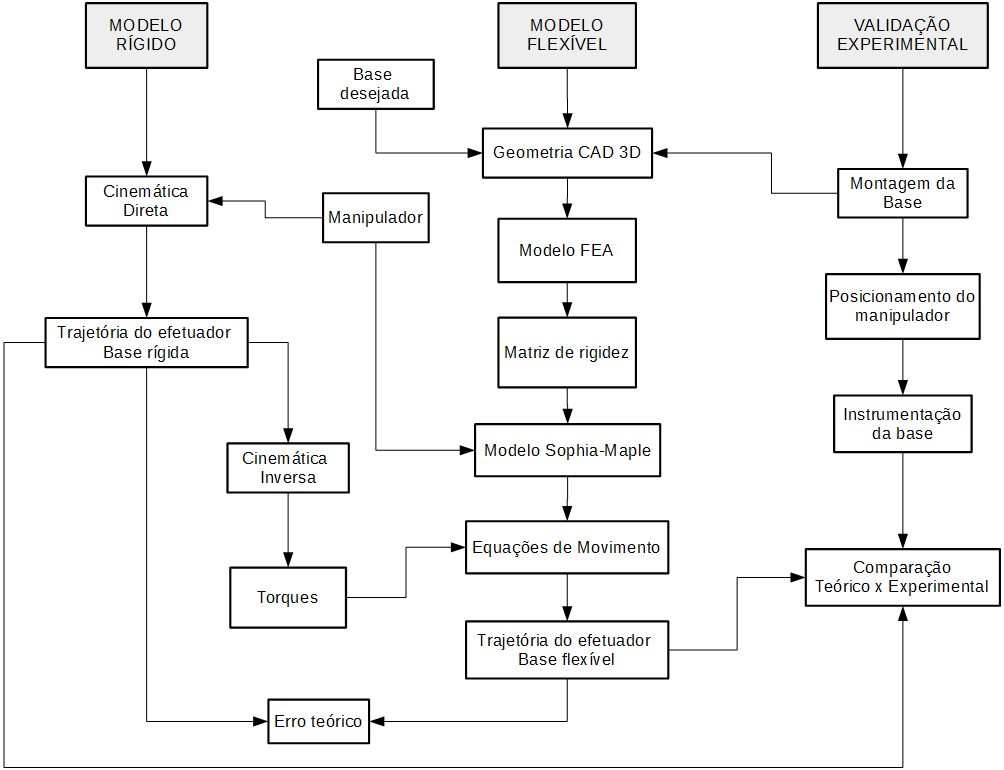
\includegraphics[width=15cm]{figs/diagrama.PNG}
\caption{Diagrama de etapas do método, Fonte: Autoria própria}
\label{fig::diagrama}
\end{figure}

\section{Fase 1: Pesquisa e viabilidade técnica}

Os primeiros 12 meses da primeira fase do projeto EMMA estudaram o Estado da
Arte para robôs de serviço, de pequeno a médio porte, utilizados em processos de
revestimento por HVOF.
A partir daí possibilitou-se o estudo da viabilidade técnica de se trasportar e
posicionar um robô dentro do espaço confinado de uma turbina, a fim de realizar
a manutenção do revestimento das pás. A figura~\ref{fig::turbina}
apresenta um desenho da turbina da Usina Hidrelétrica de Jirau-RO, onde o
protótipo EMMA será aplicado.

\begin{figure}[h!]
\centering
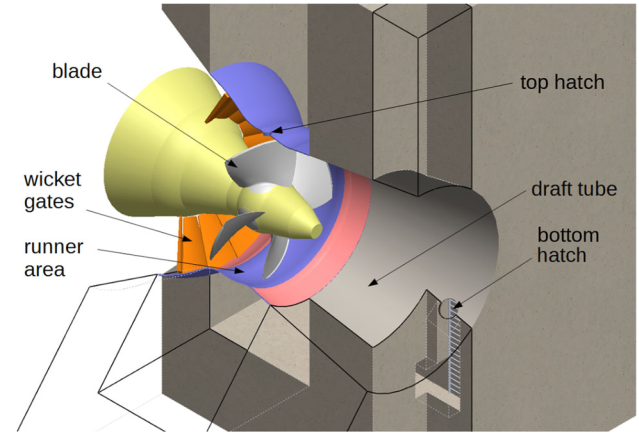
\includegraphics[width=10cm]{figs/turbina.PNG}
\caption{Turbina tipo Kaplan da UHE-Jirau, Fonte:~\citet{Freitas2017}}
\label{fig::turbina}
\end{figure}

Nesta etapa atestou-se a viabilidade da solução utilizando-se o acesso da
escotilha inferior para entrada do manipulador e dos equipamentos necessários
para montagem do sistema. 

Escolheu-se o modelo MOTOMAN MH12, da fabricante YASKAWA -- um manipulador
antropomórfico que contém 6 juntas de rotação em cadeia aberta -- por ser capaz
de entrar pelo acesso de escotilha e atender aos requisitos impostos pelo
processo de revestimento.

Definiu-se também a base sendo composta por seções modulares a serem montadas no interior da turbina para formar uma estrutura que  fornece 3 graus de liberdade para o posicionamento do robô em frente às
pás. Os módulos são compostos por perfis de alumínio estrutural e trilho,
formando uma junta prismática. Dois trilhos sobrepostos por meio de uma junta
rotacional, conferem os graus de liberdade necessários, numa configuração PRP
(Prismático-Rotacional-Prismático).
Braços de ancoragem com terminação em bases magnéticas ou copos de sucção são distribuídos a partir da
base para se obter maior rigidez da estrutura. 

A figura~\ref{fig::modulo} ilustra o o conceito da estrutura que forma a base e
destaca a composição de dois módulos que compõem a esturura.

\begin{figure}[h!]
\centering
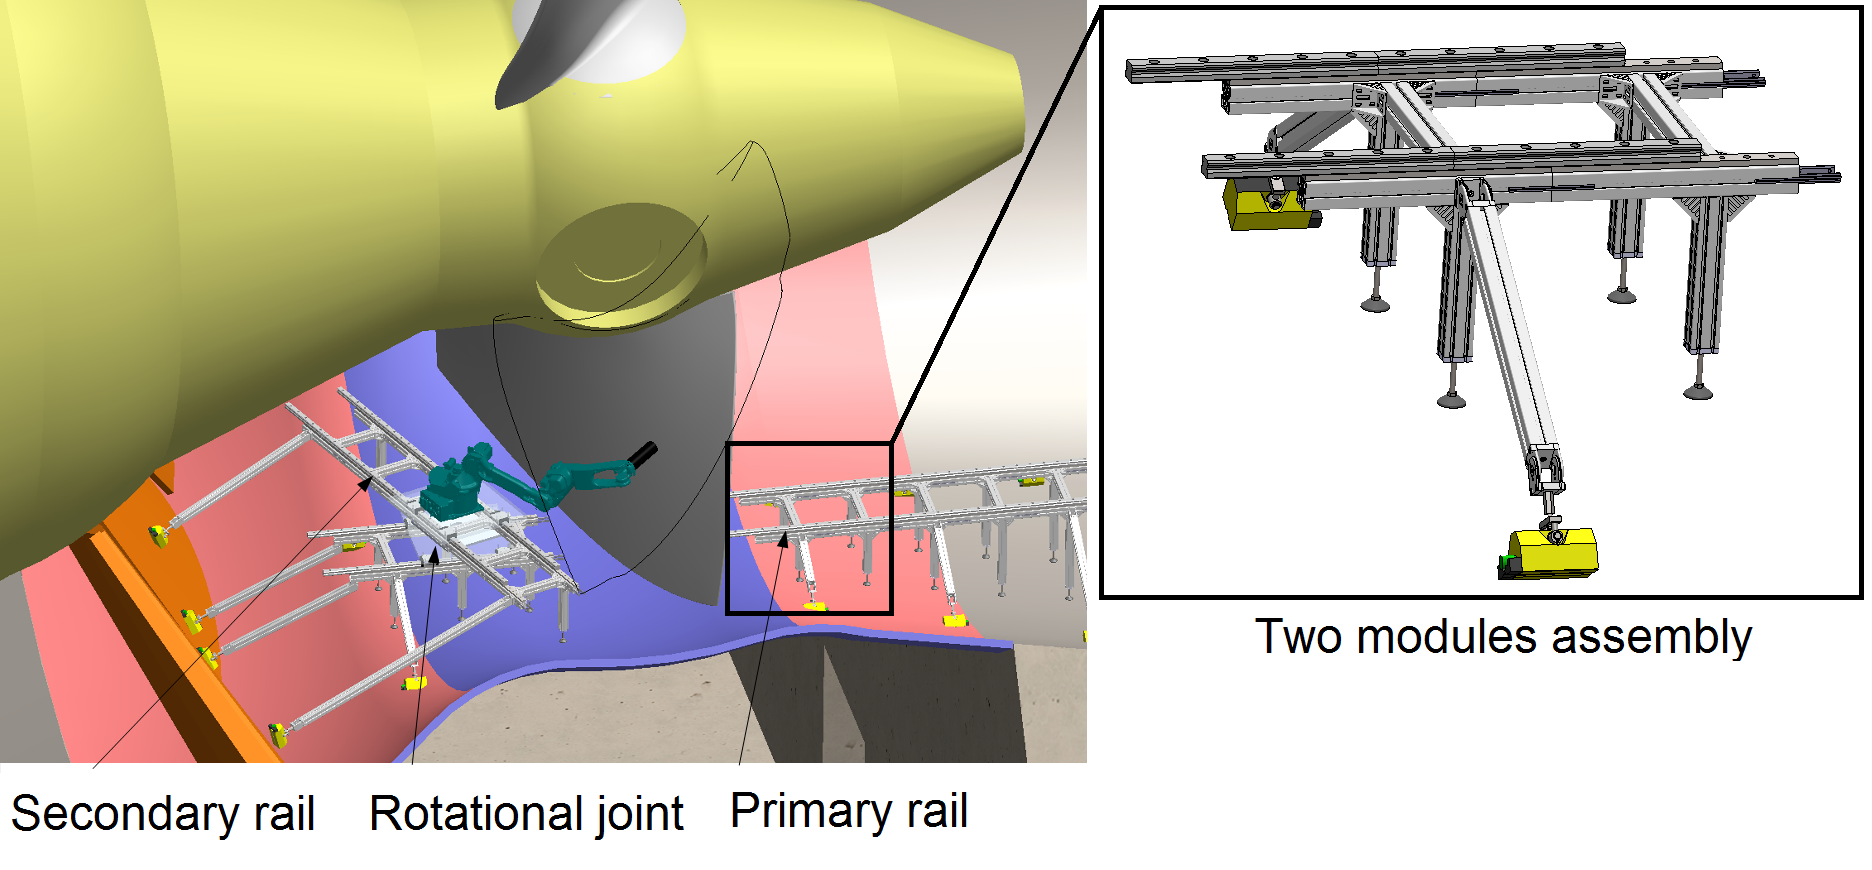
\includegraphics[width=12cm]{figs/modulo.PNG}
\caption{Base com o robô e módulo em detalhe, Fonte:~\citet{Freitas2017}}
\label{fig::modulo}
\end{figure}

\section{Fase 2: Detalhamento e simulações}

A segunda fase do projeto EMMA iniciou-se em Julho de 2016. Esta fase tem o
objetivo de detalhar a solução proposta, a fim de implementá-la ao final
do projeto, com um primeiro protótipo fabricado. Nesta etapa será incluído o
modelo de base flexível que auxiliará no dimensionamento da estrutura e dos braços de
ancoragem, considerando as cargas dinâmicas do manipulador. 

Nesta etapa destaca-se também o modelamento da geometria em CAD de diferentes
configurações de base, uma para cada posição do robô e as simulações por MEF
para obtenção da Matriz de Rigidez em função dessas posições. 

Simulações no modelo dinâmico do Sophia-Maple permitirão avaliar a influência de
diferentes configurações de base, por fornecem diferentes Matrizes de Rigidez.

Obtém-se portanto a trajetória pelo modelo flexível, o que permite verificar seu impacto no cumprimento dos requisitos de trajetória e velocidade
que o processo de revestimento HVOF requer.

\begin{figure}
\centering
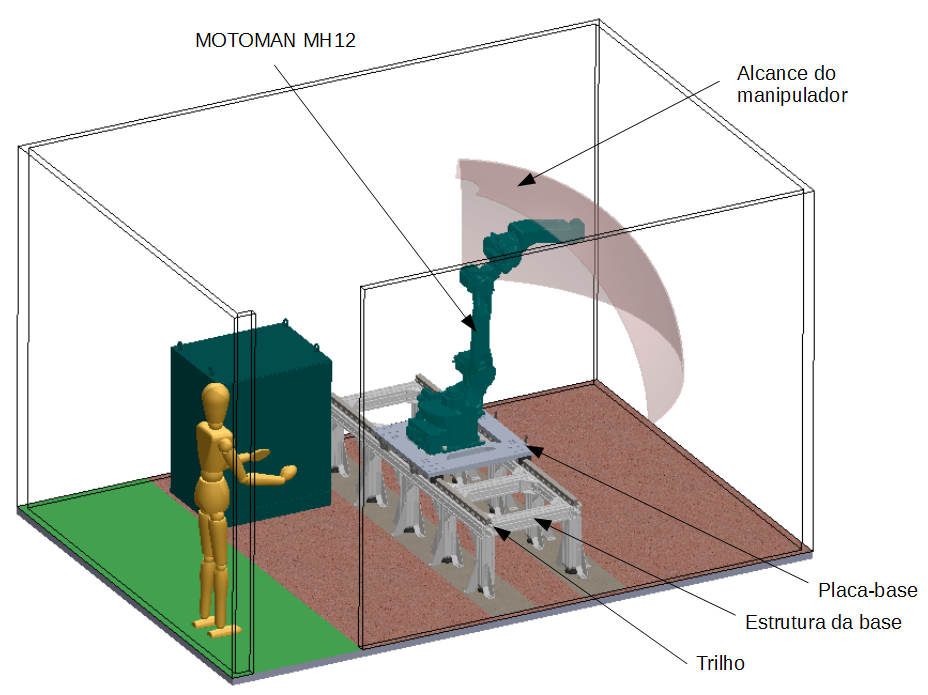
\includegraphics[width=10cm]{figs/sala_testes.PNG}
\caption{Sala de testes do manipulador, Fonte: Autoria própria}
\label{fig::base_teste}
\end{figure}

\section{Fase 3: Experimento e resultados}

O porjeto EMMA prevê uma etapa de testes de controle, trajetória, segurança,
software, interface de usuário e da base do robô. Para isso, foi montado um
laboratório de testes na empresa THIRTEEN ROBOTICS, para instalação do
manipulador em uma estrutura similar à projetada para a solução
\textit{in situ}.
Acelerômetros instalados na estrutura e alinhados com um sistema de referência
permitirão avaliar as acelerações em cada direção.
Uma trajetória idêntica a utilizada nas simulações dos modelos teóricos será
programada. Os dados de acelerações ao longo do tempo em que o robô realiza a
tarefa serão guardados e tratados para comparação com os outros
modelos.

\section{Fase 4: Discussão, redação e revisão}

A fase 4 compreende a etapa de discussão dos resultados obtidos, levando a
considerações sobre a efetividade do método proposto e trabalhos futuros.
Reserva-se esta etapa também para a revisão e redação da dissertação, e
formatação final do documento.



